% Template for PLoS
% Version 3.5 March 2018
%
% % % % % % % % % % % % % % % % % % % % % %
%
% -- IMPORTANT NOTE
%
% This template contains comments intended 
% to minimize problems and delays during our production 
% process. Please follow the template instructions
% whenever possible.
%
% % % % % % % % % % % % % % % % % % % % % % % 
%
% Once your paper is accepted for publication, 
% PLEASE REMOVE ALL TRACKED CHANGES in this file 
% and leave only the final text of your manuscript. 
% PLOS recommends the use of latexdiff to track changes during review, as this will help to maintain a clean tex file.
% Visit https://www.ctan.org/pkg/latexdiff?lang=en for info or contact us at latex@plos.org.
%
%
% There are no restrictions on package use within the LaTeX files except that 
% no packages listed in the template may be deleted.
%
% Please do not include colors or graphics in the text.
%
% The manuscript LaTeX source should be contained within a single file (do not use \input, \externaldocument, or similar commands).
%
% % % % % % % % % % % % % % % % % % % % % % %
%
% -- FIGURES AND TABLES
%
% Please include tables/figure captions directly after the paragraph where they are first cited in the text.
%
% DO NOT INCLUDE GRAPHICS IN YOUR MANUSCRIPT
% - Figures should be uploaded separately from your manuscript file. 
% - Figures generated using LaTeX should be extracted and removed from the PDF before submission. 
% - Figures containing multiple panels/subfigures must be combined into one image file before submission.
% For figure citations, please use "Fig" instead of "Figure".
% See http://journals.plos.org/plosone/s/figures for PLOS figure guidelines.
%
% Tables should be cell-based and may not contain:
% - spacing/line breaks within cells to alter layout or alignment
% - do not nest tabular environments (no tabular environments within tabular environments)
% - no graphics or colored text (cell background color/shading OK)
% See http://journals.plos.org/plosone/s/tables for table guidelines.
%
% For tables that exceed the width of the text column, use the adjustwidth environment as illustrated in the example table in text below.
%
% % % % % % % % % % % % % % % % % % % % % % % %
%
% -- EQUATIONS, MATH SYMBOLS, SUBSCRIPTS, AND SUPERSCRIPTS
%
% IMPORTANT
% Below are a few tips to help format your equations and other special characters according to our specifications. For more tips to help reduce the possibility of formatting errors during conversion, please see our LaTeX guidelines at http://journals.plos.org/plosone/s/latex
%
% For inline equations, please be sure to include all portions of an equation in the math environment.  For example, x$^2$ is incorrect; this should be formatted as $x^2$ (or $\mathrm{x}^2$ if the romanized font is desired).
%
% Do not include text that is not math in the math environment. For example, CO2 should be written as CO\textsubscript{2} instead of CO$_2$.
%
% Please add line breaks to long display equations when possible in order to fit size of the column. 
%
% For inline equations, please do not include punctuation (commas, etc) within the math environment unless this is part of the equation.
%
% When adding superscript or subscripts outside of brackets/braces, please group using {}.  For example, change "[U(D,E,\gamma)]^2" to "{[U(D,E,\gamma)]}^2". 
%
% Do not use \cal for caligraphic font.  Instead, use \mathcal{}
%
% % % % % % % % % % % % % % % % % % % % % % % % 
%
% Please contact latex@plos.org with any questions.
%
% % % % % % % % % % % % % % % % % % % % % % % %

\documentclass[10pt,letterpaper]{article}
\usepackage[top=0.85in,left=2.75in,footskip=0.75in]{geometry}

% amsmath and amssymb packages, useful for mathematical formulas and symbols
\usepackage{amsmath,amssymb}

% Use adjustwidth environment to exceed column width (see example table in text)
\usepackage{changepage}

% Use Unicode characters when possible
\usepackage[utf8x]{inputenc}

% textcomp package and marvosym package for additional characters
\usepackage{textcomp,marvosym}

% cite package, to clean up citations in the main text. Do not remove.
\usepackage{cite}

% Use nameref to cite supporting information files (see Supporting Information section for more info)
\usepackage{nameref,hyperref}

% line numbers
\usepackage[right]{lineno}

% ligatures disabled
\usepackage{microtype}
\DisableLigatures[f]{encoding = *, family = * }

% color can be used to apply background shading to table cells only
\usepackage[table]{xcolor}

% array package and thick rules for tables
\usepackage{array}

% multirow for multiple row tables. 
\usepackage{multirow}



% create "+" rule type for thick vertical lines
\newcolumntype{+}{!{\vrule width 2pt}}

% create \thickcline for thick horizontal lines of variable length
\newlength\savedwidth
\newcommand\thickcline[1]{%
  \noalign{\global\savedwidth\arrayrulewidth\global\arrayrulewidth 2pt}%
  \cline{#1}%
  \noalign{\vskip\arrayrulewidth}%
  \noalign{\global\arrayrulewidth\savedwidth}%
}

% \thickhline command for thick horizontal lines that span the table
\newcommand\thickhline{\noalign{\global\savedwidth\arrayrulewidth\global\arrayrulewidth 2pt}%
\hline
\noalign{\global\arrayrulewidth\savedwidth}}


% Remove comment for double spacing
%\usepackage{setspace} 
%\doublespacing

% Text layout
\raggedright
\setlength{\parindent}{0.5cm}
\textwidth 5.25in 
\textheight 8.75in

% Bold the 'Figure #' in the caption and separate it from the title/caption with a period
% Captions will be left justified
\usepackage[aboveskip=1pt,labelfont=bf,labelsep=period,justification=raggedright,singlelinecheck=off]{caption}
\renewcommand{\figurename}{Fig}

% Use the PLoS provided BiBTeX style
\bibliographystyle{plos2015}

% Remove brackets from numbering in List of References
\makeatletter
\renewcommand{\@biblabel}[1]{\quad#1.}
\makeatother



% Header and Footer with logo
\usepackage{lastpage,fancyhdr,graphicx}
\DeclareGraphicsExtensions{.pdf,.png}   
\usepackage{epstopdf}
%\pagestyle{myheadings}
\pagestyle{fancy}
\fancyhf{}
%\setlength{\headheight}{27.023pt}
%\lhead{\includegraphics[width=2.0in]{PLOS-submission.eps}}
\rfoot{\thepage/\pageref{LastPage}}
\renewcommand{\headrulewidth}{0pt}
\renewcommand{\footrule}{\hrule height 2pt \vspace{2mm}}
\fancyheadoffset[L]{2.25in}
\fancyfootoffset[L]{2.25in}
\lfoot{\today}

%% Include all macros below

\newcommand{\lorem}{{\bf LOREM}}
\newcommand{\ipsum}{{\bf IPSUM}}

\usepackage{xr}
\externaldocument{si}


%% END MACROS SECTION


\begin{document}
\vspace*{0.2in}

% Title must be 250 characters or less.
\begin{flushleft}
{\Large
\textbf\newline{Joint modelling of aggregated incidence data and point prevalence surveys for malaria mapping} % Please use "sentence case" for title and headings (capitalize only the first word in a title (or heading), the first word in a subtitle (or subheading), and any proper nouns).
}
\newline
% Insert author names, affiliations and corresponding author email (do not include titles, positions, or degrees).
\\
Tim C.D. Lucas*\textsuperscript{1}, Anita Nandi\textsuperscript{1}, Michele Nguyen\textsuperscript{1}, Susan Rumisha \textsuperscript{1}, Rosalind Howes \textsuperscript{1}, Katherine E. Battle \textsuperscript{1}, Penelope Hancock \textsuperscript{1}, Andre Python \textsuperscript{1}, Ewan Cameron\textsuperscript{1}, Pete Gething\textsuperscript{1} and Daniel J. Weiss\textsuperscript{1}
\\
\bigskip
\textbf{1} BDI, Oxford
\\
\bigskip

% Insert additional author notes using the symbols described below. Insert symbol callouts after author names as necessary.
% 
% Remove or comment out the author notes below if they aren't used.
%

% Current address notes



% Use the asterisk to denote corresponding authorship and provide email address in note below.
* timcdlucas@gmail.com

\end{flushleft}
% Please keep the abstract below 300 words
\section*{Abstract}
As malaria incidence decreases and more contries move towards elimination, maps of malaria risk in low prevalence areas are becoming increasingly needed.
However, traditional mapping using prevalence point-surveys are often ineffective in low prevalence areas due to low statistical power and a lack of data.
Therefore, models must be developed that can estimate risk at high spatial resolution from surveillance data that reports incidence aggregated to a geographic polygon.
Current models formulated for polygon incidence data suffer from lower statistical power for learning relationships between malaria risk and environmental covariates.
Here we present a joint model that uses both polygon incidence and prevalence point-surveys.


% Please keep the Author Summary between 150 and 200 words
% Use first person. PLOS ONE authors please skip this step. 
% Author Summary not valid for PLOS ONE submissions.   
\section*{Author summary}
Todo


\linenumbers

% Use "Eq" instead of "Equation" for equation citations.
%%%%%%%%%%%%%%%%%%%%%%%%%%%%%%%%%%%%%%%%%%%%%%%%%%%%%%%%%%%%%%%%%%%%%%%%%%%%%%%%%%%%%%%%%%%%%%%%%%%%%
\section*{Introduction}
%%%%%%%%%%%%%%%%%%%%%%%%%%%%%%%%%%%%%%%%%%%%%%%%%%%%%%%%%%%%%%%%%%%%%%%%%%%%%%%%%%%%%%%%%%%%%%%%%%%%%


% Glossary
% Models:
%   Joint model
%   Polygon-only model
%   Point-only model
% Data:
%   Prevalence point-surveys
%   Polygon incidence
% Variables:
%   Pixel-level prevalence
%   Polygon-level incidence
%   Pixel-level incidence

Global malaria incidence has decreased dramatically over the last 20 years \cite{abajobir2017global, bhatt2015effect}.
This decrease has been accompanied by a strategic shift towards aiming for elimination in low incidence countries \cite{world2016world, newby2016path}.
Accurate, high-resolution maps of malaria risk are vital in countries in the elimination and pre-elimination phases \cite{sturrock2016mapping, cohen2017mapping}.
However, mapping malaria in low burden countries presents new challenges as traditional mapping of prevalence \cite{gething2011new, bhatt2017improved, gething2012long, bhatt2015effect} using cluster-level surveys and model-based geostatistics are not necessarily effective in these areas \cite{sturrock2016mapping, sturrock2014fine}.
In low burden areas, very large sample sizes are needed before a prevalence survey is informative because so few individuals have parasitaemia that most sample points will have no cases.
As a result, large, countrywide surveys of prevalence, such as DHS or MIS, are rare in low burden countries due to costs and percieved low utility \cite{dhs}.
We therefore need new data sources and associated statistical methods.

%Despite major reductions in incidence over the last fifteen years, malaria still causes millions of deaths and loads of DALYs annually \cite{abajobir2017global}.
%Elimination of malaria, country-by-county has become a central goal in the global malaria strategy \cite{world2016world}.
%Elimination of malaria requires high resolution maps of malaria risk, in low prevalence areas in order to optimise interventions and minimise costs \cite{sturrock2016mapping}.

%cohen2017mapping Different metrics are useful for different things. Most maps use prevalence. Govts do use maps.

Routine surveillance data, of malaria case counts, is becoming more widely available and of better quality \cite{sturrock2016mapping, ohrt2015information, cibulskis2011worldwide}.
Surveillance data is commonly aggregated from information collected at healthcare facilities or by community health workers, reporting the number of cases that occurred within a certain geographic or administrative region defined by a polygon.
This polygon incidence data can be more sensitive than prevalence point-surveys in low transmission areas as the entire public health system is being used to passively monitor disease risk \cite{cibulskis2011worldwide}.
Furthermore, polygon incidence data is also often timely, with reports being released annually or monthly with little lag, while countrywide collection of prevalence point-surveys are both rare and often released one to two years after field data collection is completed.
However, the unstructured nature of data collection and reporting of polygon incidence data from national disease surveillance systems means that dealing with biases and data gaps is an ongoing research priority \cite{battle2016treatment, cibulskis2011worldwide}.

%however surveillance data is sometimes high quality in these areas
%pixel level maps from aggregates data is difficult (sturrock2014fine, wilson2017pointless, law2018variational, others)
%not much information for covariates 
%sturrock used two.
%undeveloped area of statistics but see Leon.

Disaggregation regression methods have been proposed as a way to model malaria burden using polygon-level incidence \cite{sturrock2014fine, wilson2017pointless, law2018variational, taylor2017continuous, li2012log}.
However using polygon incidence data to estimate malaria risk for high resolution maps presents several noteworthy modelling difficulties. 
%Disaggregation models aim to estimate high-resolution maps from aggregated data and are characterised by having a variable number of pixels, and therefore multiple rows of covariate data, per row of response data.
The aggregation of cases over space means that the data may be relatively uninformative, especially if the case counts are aggregated over a large or heterogenous area.
This lack of statistical power puts constraints on the models that can be fitted for example requiring variable selection and simple linear terms \cite{sturrock2014fine}.
Disaggregation models are also simply an underrepresented class of models in the statistical literature and statistical software relative to model-based geostatistical approaches.
Likewise, downscaling models are not available in popular software packages and must typically be programmed explicitly though Wilson \emph{et al.} \cite{wilson2017pointless} used an approximation to represent a downscaling model as a convolution matrix within R-INLA \cite{INLA}.
Furthermore, disaggregation models are relatively difficult to implement as they have more rows of covariate data than response data.


Given the differing strengths of prevalence point-surveys and polygon incidence data, a model that simultaneously leverages both data types has great potential to improve malaria burden mapping.
Joint modelling of the two data types could provide increased statistical power for learning relationships between malaria risk and covariates by making more data available and because point-surveys have a one-to-one relationship with gridded environmental covariates at the location and time of the survey.
Furthermore, using two complimentary datasets potentially allows better spatial coverage \cite{sturrock2016mapping}. 
One major barrier to a joint modelling approach, however, is that these two data types capture different scales.
Point surveys are a measurement of prevalence in the range $\lbrack 0, 1\rbrack$ that quantify parasite rate at a single moment. In contrast,
In contrast, routine surveillance measures incidence in the range $\lbrack 0, \infty\rbrack$ as it spans a period of time (e.g., a year) over which individuals can have multiple malaria infections..
%One approach to combining these datasets is to use a seperately estimated model that maps one scale to another such as \cite{cameron2015defining}.

%Ideal situation is to combine data
%benefits of both
%but data are on different scales
%Ewan says there's a relationship.

Here we formulate a joint model that combines polygon incidence data and prevalence point-surveys of \emph{Plasmodium falciparum} using seperate likelihoods for both data types.
We relate the differing malariometric measures by using a previously estimated relationship within the model \cite{cameron2015defining}.
We then compare results from the joint model with those made using a polygon-only, disaggregation model similar to previous models \cite{sturrock2014fine, wilson2017pointless}.
Both models are fitted to data from Indonesia, Senegal and Madagascar to provide a set of case studies with disparate geographic settings and levels of malaria endemicity.

%here we compared 3 models, point only, polygon only and joint models
%we use Madagascar and Indonesia as case studies as they have good %surveillance data and good pr data.




%%%%%%%%%%%%%%%%%%%%%%%%%%%%%%%%%%%%%%%%%%%%%%%%%%%%%%%%%%%%%%%%%%%%%%%%%%%%%%%%%%%%%%%%%%%%%%%%%%%%%
\section*{Materials and methods}
%%%%%%%%%%%%%%%%%%%%%%%%%%%%%%%%%%%%%%%%%%%%%%%%%%%%%%%%%%%%%%%%%%%%%%%%%%%%%%%%%%%%%%%%%%%%%%%%%%%%%


\subsection*{Malaria data}

We used two data sources that reflect malaria burden; prevalence point-surveys and polygon incidence data.
We selected Indonesia, Senegal and Madagascar as case examples as they all have abundant subnational surveillance data and country wide surveys from approximately the same period.
To minimise temporal effects we selected, for each country, one year of prevalence point-survey data and one year of polygon incidence data.
For Indonesia we selected polygon incidence data from 2012 that covers 380 regions, and prevalence data from 2010 to 2014 that consists of todo surveys, accounting for todo individuals.
For Senegal we selected 2015 for polygon incidence data (46 regions) and 2013 to 2017 for prevalence data (todo surveys, todo).
Finally, for Madagascar we selected 2013 for polygon incidence (110 regions) and 2011 to 2015 prevalence (todo surveys, todo individuals) data.



\subsection*{Prevalence survey data}

The prevalence point-survey data were extracted from the Malaria Atlas Project prevalence survey database \cite{bhatt2015effect, guerra2007assembling, gething2011new, pfeffer2018ma}.
As the prevalence point-surveys cover different age ranges they were standardised to an age-range of 2--10 using the model from \cite{smith2007standardizing}.
The age standardisation model gives the surveys with zero positive cases a small positive prevalence.

\subsection*{Polygon incidence data}

% (Figures~\ref{predobsmapidn}A and \ref{predobsmapsen}A)

The polygon incidence data were collated from various government reports and adjusted to a standard metric using methods defined in \cite{cibulskis2011worldwide}.
These adjustments account for underreporting of clinical cases due to lack of treatment seeking, missed case reports, and cases that sought medical attention outside the public health systems \cite{battle2016treatment}.
Where species specific reports were given, these were used, and in reports that did not distinguish between species of \emph{Plasmodium} the national estimate of the ratio between \emph{P. falciparum} and \emph{P. vivax} cases were used to estimate \emph{P. falciparum} only cases.



\subsection*{Population data}

Raster surfaces of population for the years 2005, 2010 and 2015, were created using a hybrid of data from GPWv4 \cite{gpw4} and WorldPop \cite{tatem2017worldpop}, with the latter taking priority for those pixels where both had population data. 
Final population rasters were created by linear interpolation of the surrounding five-yearly rasters.
Finally, for each year, national population estimates from the UN were raked over the interpolated population surfaces. 

\subsection*{Covariate data}

We considered an initial suite of environmental and anthropological covariates, at a resolution of approximately $5 \times 5$ kilometres at the equator that included land surface temperature annual mean and standard deviation \cite{LST}, enhanced vegetation index \cite{TCB}, mosquito temperature suitability index \cite{weiss2014air}, elevation \cite{SRTMElev}, tassel cap brightness \cite{TCB}, tassel cap wetness \cite{TCB}, accessibility to cities \cite{weiss2018global}, night lights \cite{} and proportion of urban land cover \cite{}. % change to table
Some covariates were log-transformed to remove skewness or removed due to multicollineariy with other predictor variables using the threshold of 0.8. % think we decided this on indonesia data only. Sen is currently 0.81... just a bit messy.
The covariates were standardised to have a mean of zero and a standard deviation of one.

\subsection*{The model}

We compared three models 1) a joint model using both  prevalence point-surveys and polygon incidence data as the response variable 2) a submodel using only polygon incidence data and 3) a benchmark submodel using only prevalence point-survey data. 
The models were implemented and fitted in R \cite{R} using Template Model Builder \cite{TMB} which allows a Laplace approximation of the posterior to be calculated.

The full, joint likelihood model is described as follows. 
Values at the aggregate, polygon level are given the subscript $a$ while pixel or point level variables are indexed with $b$.
The polygon incidence case count data, $y_j$ is given a Poisson likelihood

$$y_a \sim \operatorname{Pois}(i_a\mathrm{pop_a})$$

where $i_a$ is the estimated polygon incidence rate and $\mathrm{pop_a}$ is the observed polygon population-at-risk.

The prevalence point-survey data, $z_b$, is given a binomial likelihood

$$z_b \sim \operatorname{Binom}(p_b, n_b) $$

where $p_b$ is the estimated prevalence and $n_b$ is the observed survey sample size. 

The two quantities are linked to each other and to the predictor variables by the following system of equations.

$$i_a = \frac{ \sum_{b \in a}(i_b \mathrm{pop}_b)}{\sum_{b \in a}\mathrm{pop}_b} $$

where

$$i_b = \exp(\alpha)\mathrm{PrevInc}(p_b).$$

Here $\mathrm{PrevInc}$ is a function from a previously fitted model \cite{cameron2015defining} 
$$\mathrm{PrevInc}: f\left(p_b\right) = 2.616p_b - 3.596{p_b}^2 + 1.594{p_b}^3.$$
$\alpha$ is a parameter to be fitted that adjusts the previously fitted function.

The linear predictor of the model, $\eta_b$, is related to prevalence by a typical logit link function.

$$p_b = \operatorname{logit}^{-1}(\eta_b)$$


The form of the link function means we get predictions of prevalence and incidence simultaneously whether we used both data types or just one.
The linear predictor is composed of a global intercept, $b_0$, and a prevalence survey only intercept $b_p$ where the indicator function, $\mathbf{1}_p$ denotes that this term is zero except when a prevalence point survey is being considered.
The linear predictor also includes covariates, $X$, and a vector of regression coefficients $\beta$.
Finally we include a spatial, Gaussian random field and two iid random effects.

$$\eta_b = \beta_0 + \mathbf{1}_p\beta_p +  \beta X  + u(s, \rho, \sigma_u) + v_j(\sigma_v) + w_i(\sigma_w)$$

The Gaussian spatial effect $u(s, \rho, \sigma_u)$ has a Mat\'ern covariance function and two hyper parameters: $\rho$, the nominal range (beyond which correlation is $< 0.1$) and $\sigma_u$, the marginal standard deviation.
The first iid random effect, $v_j \sim \operatorname{Norm}(0, \sigma_v)$,  was grouped by polygon, with all pixels and point surveys within polygon $j$ being grouped together.
This random effect modelled both missing covariates and extra-Poisson sampling error. 
The second iid random effect, $w_i \sim \operatorname{Norm}(0, \sigma_w)$, was applied to each point survey.
This effect modelled extra-binomial sampling noise.
As such, this random effect is not included in the predicted uncertainty in the incidence or prevalence layers.
However, it is included in predictions of out-of-sample point surveys.
The randoms effects are all integrated out during the TMB model fitting.
The hyperparameters are fitted during model fitting using empirical Bayes.
In this empirical Bayes scheme the hyperparameters are learned from the data but are treated as point estimates rather than the model using the full posterior of the hyperparameters.



Finally, we complete the model by setting priors on the parameters $\beta_0, \beta_p, \beta, \rho$ and $\sigma_u$, $\sigma_v$ and $\sigma_w$.
We assigned $\rho$ and $\sigma_u$ a joint penalised complexity prior \cite{fuglstad2018constructing} such that $P(\rho < \zeta) = 0.00001$ and $P(\sigma_u > 1) = 0.00001$.
We used different $\zeta$ values for each country: Indonesia $\zeta = 3$, Senegal $\zeta = 1$ and Madagascar $\zeta = 1$.
We believe that a large proportion of the variance of malaria prevalence and incidence cannot be explained by a linear combination of the covariates selected \cite{bhatt2017improved}, so we set this prior such that the random field could explain most of the range of the data.

We assigned $\sigma_v$ a penalised complexity prior \cite{simpson2017penalising} such that $P(\sigma_v > 0.05) = 0.0000001$
This was based on a comparison of the variance of Poisson random variables, with rates given by the number of cases observed, and an independently derived upper and lower bound for the case counts using the approach defined in \cite{cibulskis2011worldwide}.
We found that an iid effect with a standard deviation of 0.05 is able to account for the discrepancy between the assumed Poisson error and the independently derived error.
We assigned $\sigma_w$ a penalised complexity prior such that $P(\sigma_w > 0.3) = 0.0000001$. 
This was chosen by finding the maximum difference in prevalence between point-surveys (with a sample size greater than 500 individuals) within the same raster pixel.
The differences between points within the same pixel can only be accounted for by the binomial error and this iid effect.
Given that the error on a prevalence estimate with sample size greater than 500 is quite small, the iid effect needs to be able to explain this difference.

%\begin{figure}[t!]
%% to be removed before submission
%\centering
%
%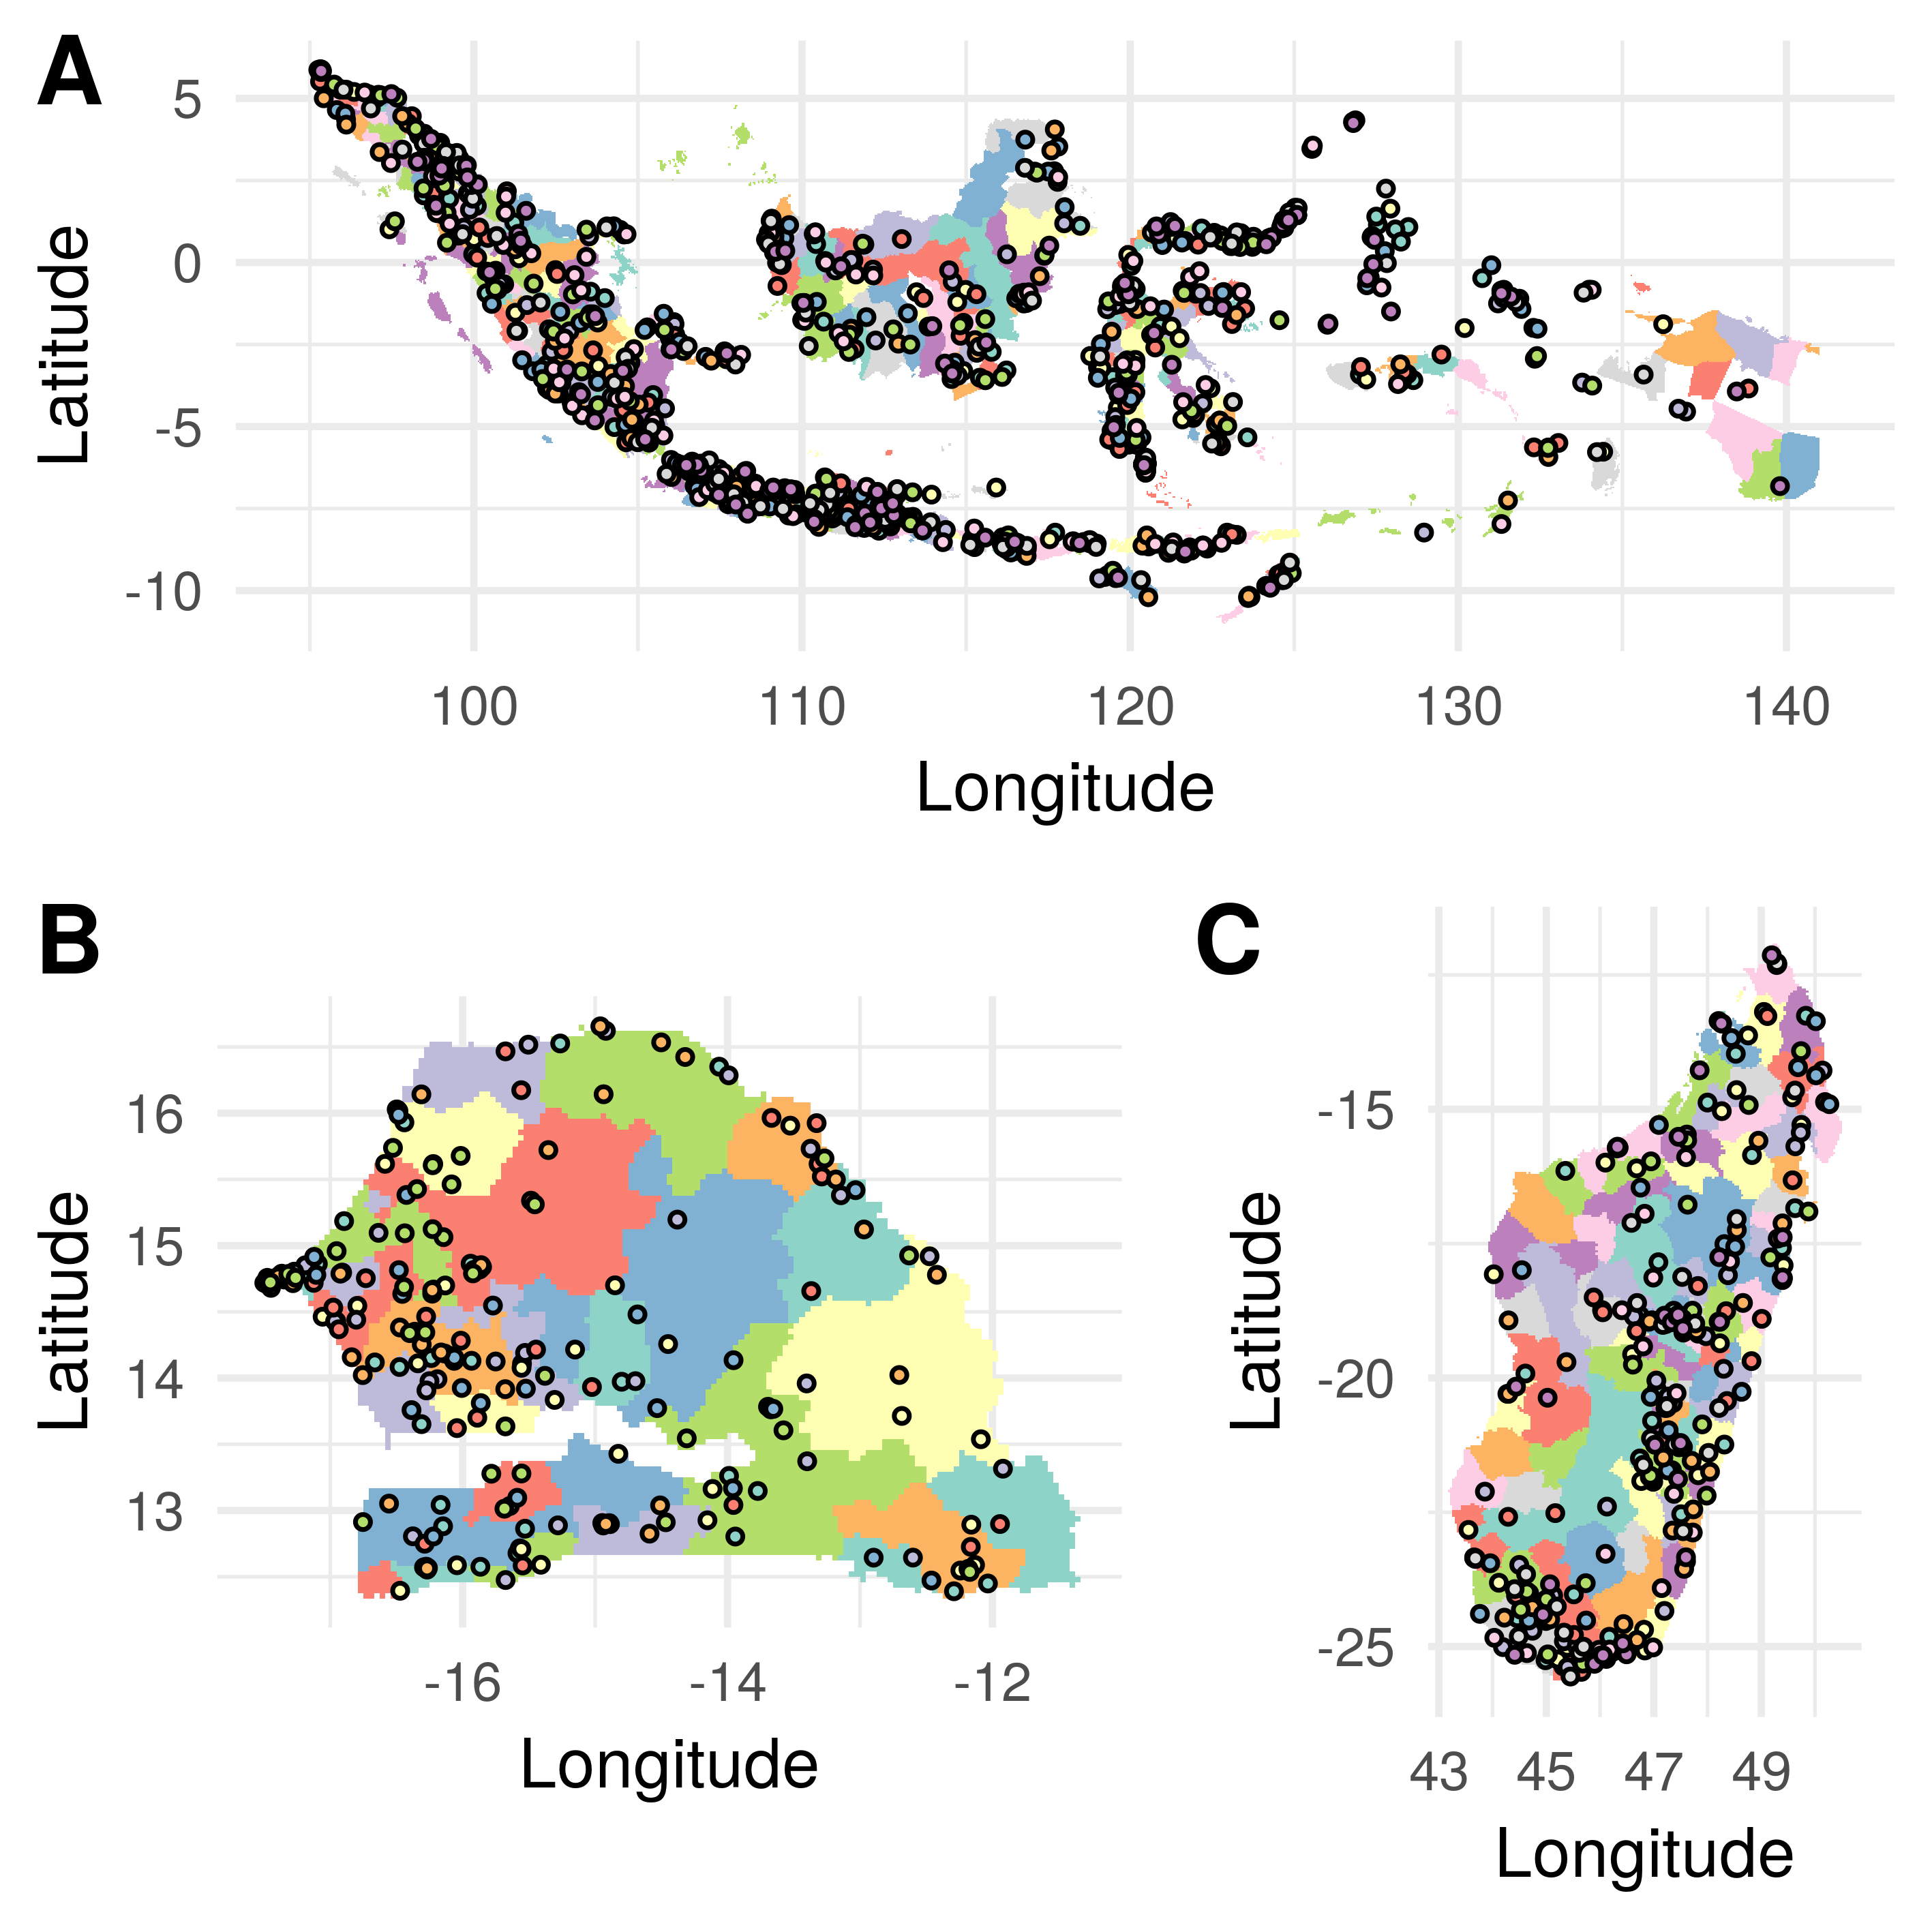
\includegraphics[width = 0.9\textwidth]{figures/random_crossvalidation_full.png} %\caption{Indonesia random crossvalidation} 
%
%\caption{{\bf Random cross-validation scheme for Indonesia, Senegal and Madagascar.} The fold for both aggregated incidence data and prevalence point data is shown.}
%\label{fig:cv_random}
%\end{figure}
%
%
%\begin{figure}[!t]
%% to be removed before submission
%\centering
%
%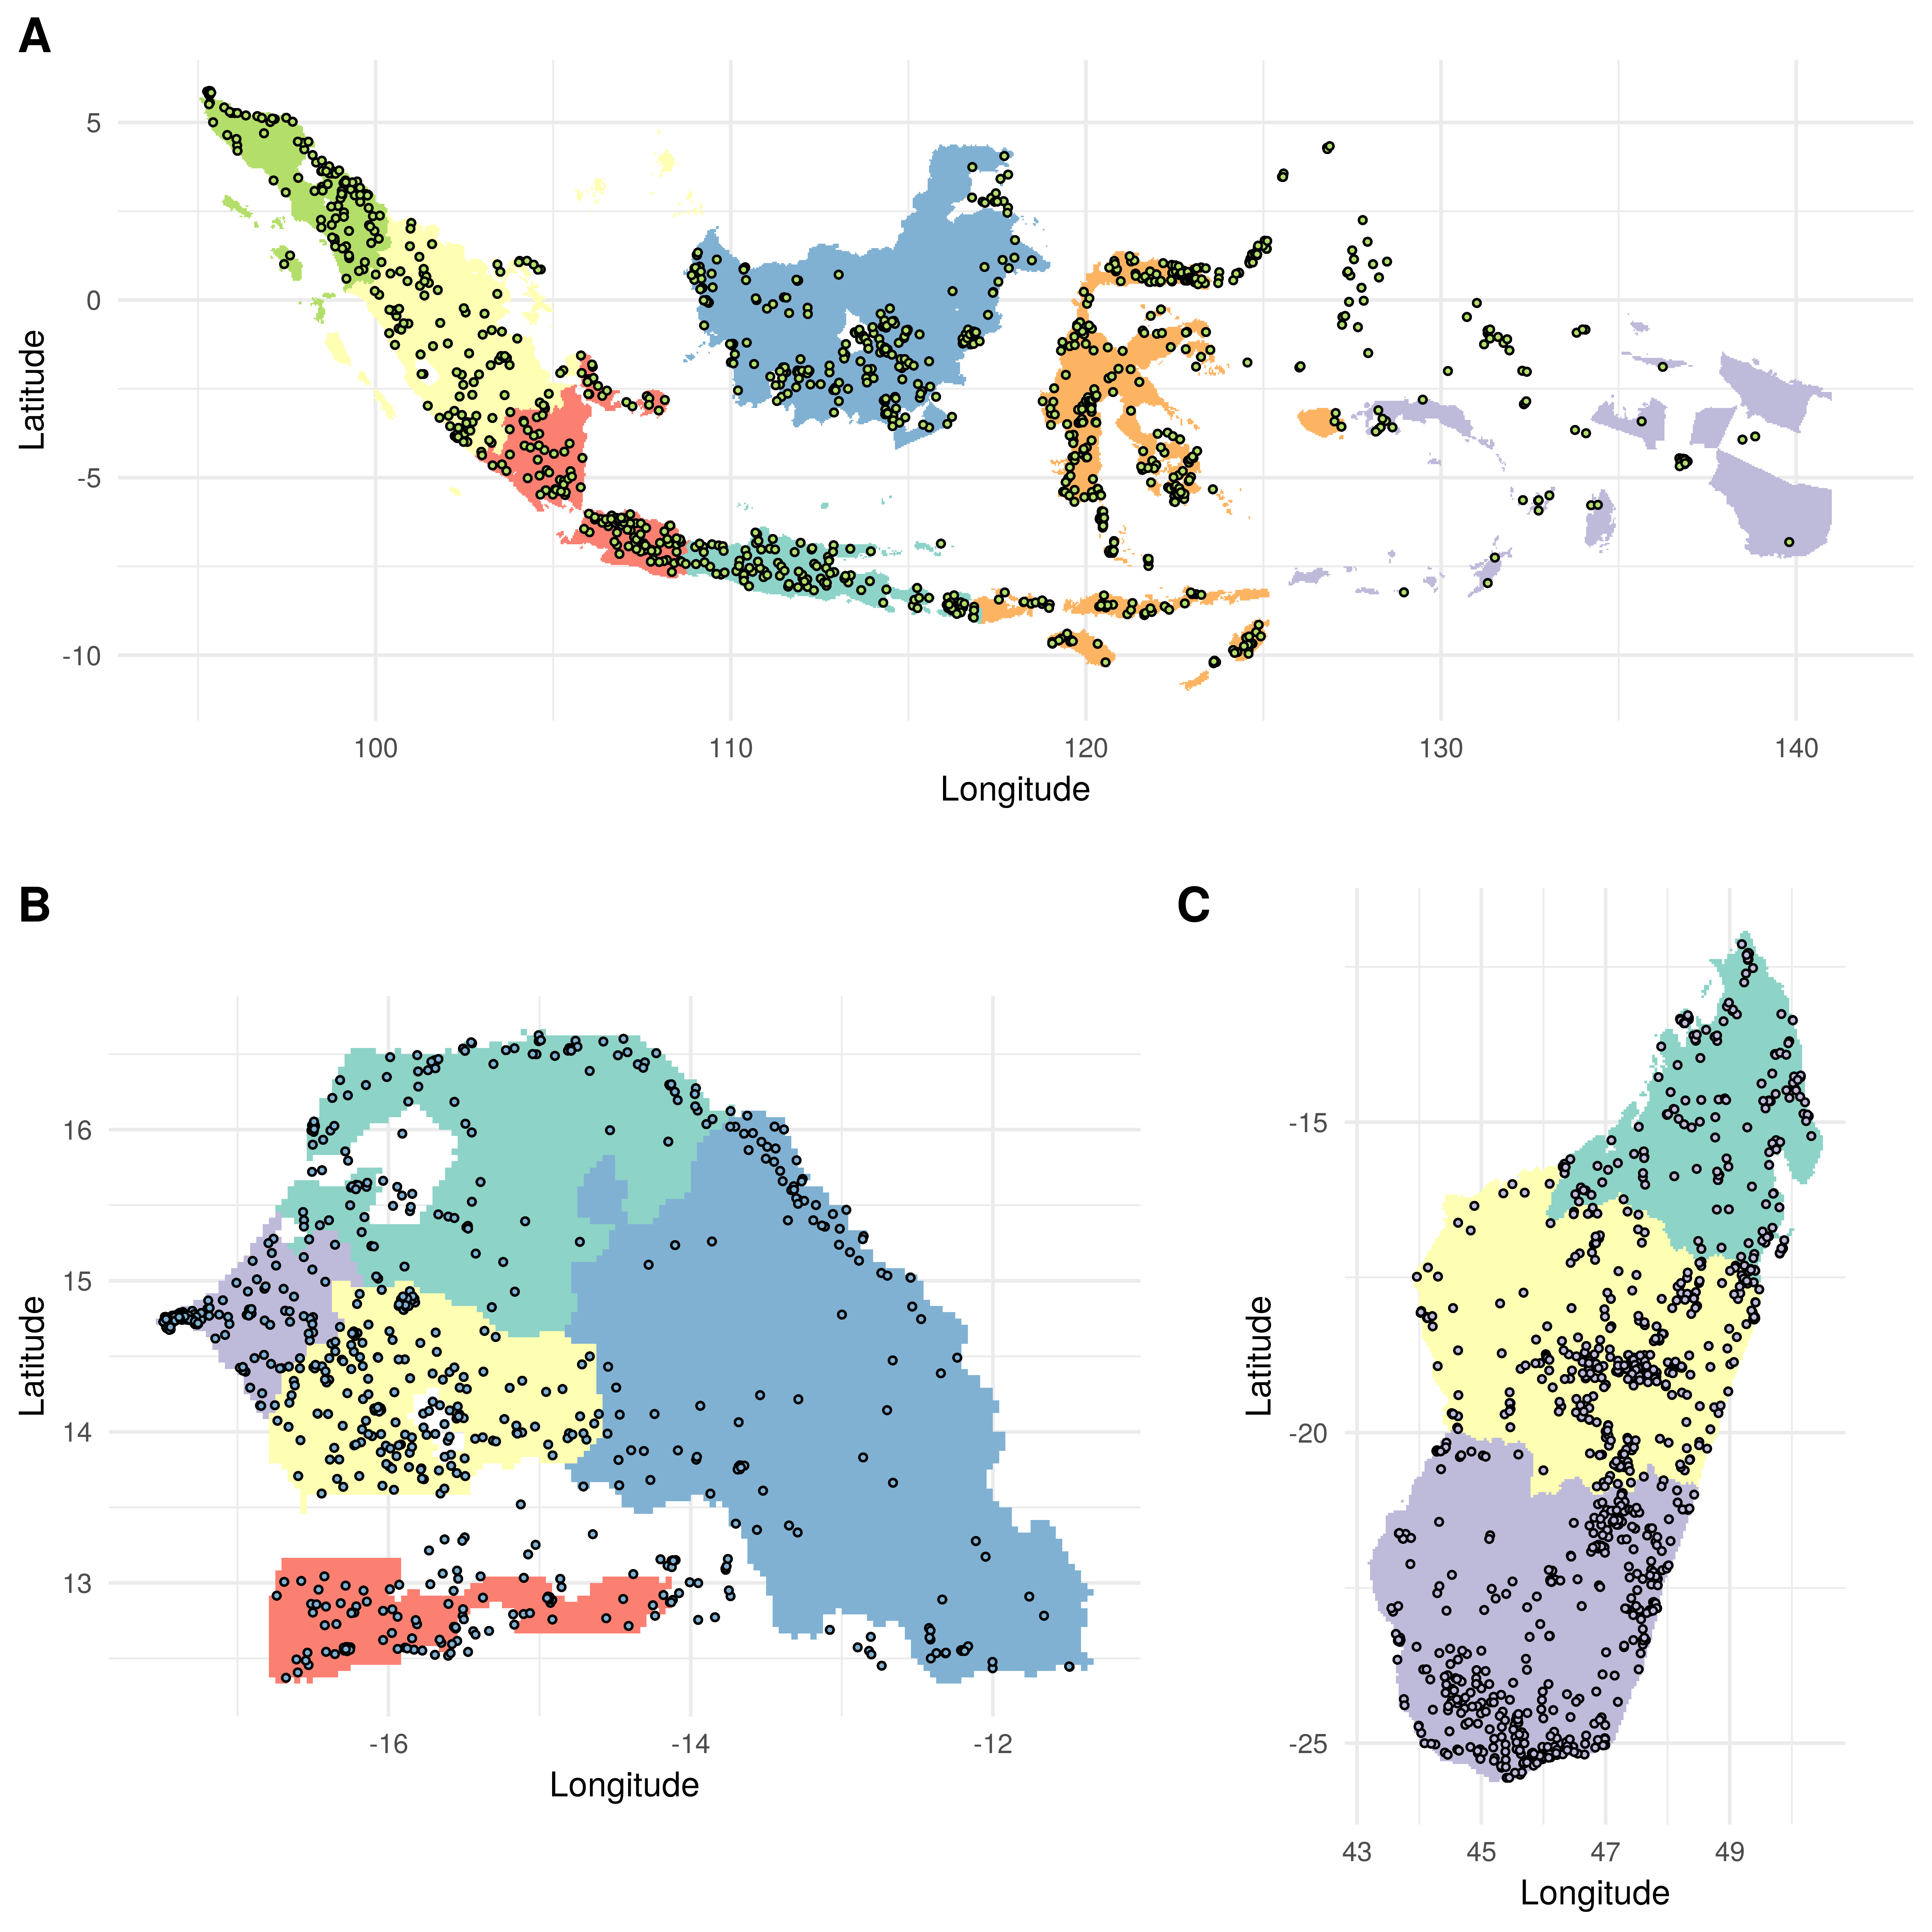
\includegraphics[width = 0.9\textwidth]{figures/spatial_crossvalidation_full.png} %\caption{Indonesia random crossvalidation} 
%
%\caption{{\bf Spatial cross-validation scheme for Indonesia, Senegal and Madagascar.} The fold for both aggregated incidence data and prevalence point data is shown.}
%\label{fig:cv_spatial}
%\end{figure}
%

The intercept was given a wide prior, $b_0 \sim \operatorname{Norm}(-2, 4)$ with a mean less than zero as we know \emph{a priori} that these countries have low or medium levels of malaria transmission.
The prevalence only intercept was given a wide, zero-mean prior, $b_0 \sim \operatorname{Norm}(0, 4)$. % check
Finally, we set regularising priors on the regression coefficients $\beta_i \sim \operatorname{Norm}(0, 0.04)$. 
Given the standardised covariates, a regression coefficient from the 95\% IQR of this distribution, and an intercept of -3, each covariate is able to predict prevalences between 0.004 and 0.27. 
This prior encodes our desire to regularise our model and and belief that the full range of malaria transmission can not be explained by a single covariate and our desire to regularise our model.
This regularisation is particularly important given the small number of observations in Senegal (n = 46) and Madagascar (n = 110).



\subsection*{Experiments}

To compare the three models we used three cross-validation schemes. 
In the first (random), the incidence data was split into ten cross-validation folds while all the prevalence data was used in each case.
%This cross-validation scheme directly addresses the question of whethe
In the second validation scheme (spatial a), the incidence data was split into spatial cross-validation folds, using k means clustering on polygon centroids, while again all prevalence points were used in all folds.
The number of folds was seven for Indonesia, five for Senegal and three for Madagascar due to their differing sizes and epidemiological settings.
This scheme is specifically testing whether the joint model can improve predictions by increasing geographic data coverage.
This situation is particularly common in continental scale models where some countries will have large DHS style surveys but little incidence data.
In the final scheme (spatial b) the data is again split spatially but the prevalence surveys from the hold-out areas are also witheld.
This scheme is testing the models' ability to predict into new areas with little information from the spatial random field.
It is therefore testing how well the models learn the parameters that relate the environment to malaria risk.

We considered the ability to predict polygon incidence correctly our main objective and our performance metric was mean absolute error (MAE).
As the models are being fitted on data on difference scales we found that observations and predictions were sometimes correlated but strongly displaced from the one-one line and therefore correlation metrics were misleading.
% Why not correlation
To assess how well the models were calibrated we considered coverage of the 80\% predictive credible intervals on the hold-out data.




\begin{table}[!t]
\begin{adjustwidth}{-2.25in}{0in} % Comment out/remove adjustwidth environment if table fits in text column.
\centering
\caption{
{\bf Summary of out-of-sample accuracy for all three cross-validation experiments.}}
\begin{tabular}{llll}
\hline
{\bf CV scheme} & {\bf Country} &  {\bf Polygons} & {\bf Joint} \\
\thickhline 
Random & Indonesia  & 13.95 &  {\bf 13.88}\\
& Senegal  & {\bf 12.41} &  12.81\\
& Zambia  & {\bf 154.59} &  154.96\\
& Madagascar  & 39.06 &  {\bf 36.36}\vspace{3mm}\\
Spatial 1 & Indonesia & {\bf 14.77} &  15.08\\
& Senegal  & {\bf 12.39} &  16.56\\
& Zambia  & {\bf 162.74} &  163.74\\
& Madagascar  & 70.72 &  {\bf 61.05}\vspace{3mm}\\
Spatial 2 & Indonesia & {\bf 14.81} &  16.36\\
& Senegal  & {\bf 12.31} &  15.91\\
& Zambia  & {\bf 135.39} &  184.14\\
& Madagascar & 67.73 &  {\bf 44.05}\\
\end{tabular}
\begin{flushleft}
Mean absolute error of predicted incidence rate against out-of-sample observed data for three countries.
\end{flushleft}
\label{table1}
\end{adjustwidth}
\end{table}





% Results and Discussion can be combined.
%%%%%%%%%%%%%%%%%%%%%%%%%%%%%%%%%%%%%%%%%%%%%%%%%%%%%%%%%%%%%%%%%%%%%%%%%%%%%%%%%%%%%%%%%%%%%%%%%%%%%
\section*{Results}
%%%%%%%%%%%%%%%%%%%%%%%%%%%%%%%%%%%%%%%%%%%%%%%%%%%%%%%%%%%%%%%%%%%%%%%%%%%%%%%%%%%%%%%%%%%%%%%%%%%%%

% Random cv

Under the random cross-validation scheme, the joint model performed best in Indonesia and Madagascar while the polygon only model performed best in Senegal (Table \ref{table1}).
The differences were relatively small in all three countries.
This lack of strong differences is highlighted by the fact that there are no clear differences in scatter plots of observed and predicted data (Figure \ref{randompredobspolyfacet}).
 


% spatial 1

Under the spatial a cross-validation scheme, the polygon only model performed best in Indonesia and Senegal while the joint model performed best in Madagascar (Table \ref{table1}).
In contrast to the random cross-validation results, the differences between models is quite strong.
Furthermore, notable difference can be seen in the scattor plots of observed and predicted values (Figure \ref{spatial2predobspolyfacet}).
In Indonesia it can be seen the the joint model is more strongly biased at low incidence values with many data points being overpredicted.
In Senegal the predictions from the joint model do not appear biased but are often far from the observed value.
However, the joint model clearly performs better in Madagascar with the polygon only model particularly struggling to predict high incidence observations correctly.


% spatial b

Under the spatial b cross-validation scheme, in which the prevalence data are spatially withheld, the polygon model again performs the best in Indonesia and Senegal while the joint model performs best in Madagascar (Table \ref{table1}).
The bias in the low incidence observations in Indonesia is no longer present (Figure \ref{spatial1predobspolyfacet}).
In Indonesia and Senegal the joint model performs worse in the spatial a cross-validation than in the spatial b cross-validation scheme.
Given that more data is being witheld in spatial b this implies that the bias caused by the prevalence points is so severe that models perform worse with this spatial information than with just information from the covariates.

\begin{figure}
% to be removed before submission
\includegraphics[width = 1.05\textwidth]{figures/random_cv_poly_facet}  
\caption{{\bf Observed-predicted plots for random cross-validation experiments.}
A) Indonesia, B) Senegal, C) Madagascar. Square root aggregated incidence (per 1,000).
Results from the standard downscaling model are shown in blue and the combined model is shown in green.
}
\label{randompredobspolyfacet}
\end{figure}


%figure 5, 6. Spat and random cv. PR vs Poly columns, countries as rows, model as colour?


\begin{figure}
% to be removed before submission
\includegraphics[width = 1.05\textwidth]{figures/spatialkeeppr_cv_poly_facet}  
\caption{{\bf Observed-predicted plots for spatial a cross-validation experiments where all prevalence points are used in model fitting.}
A) Indonesia, B) Senegal, C) Madagascar. Square root aggregated incidence (per 1,000).
Results from the standard downscaling model are shown in blue and the combined model is shown in green.
}
\label{spatial2predobspolyfacet}
\end{figure}



\begin{figure}
% to be removed before submission
\includegraphics[width = 1.05\textwidth]{figures/spatial_cv_poly_facet} 
\caption{{\bf Observed-predicted plots for spatial b cross-validation experiments where prevalence points are spatially witheld.}
A) Indonesia, B) Senegal, C) Madagascar. Square root aggregated incidence (per 1,000).
Results from the standard downscaling model are shown in blue and the combined model is shown in green.
}
\label{spatialpredobspolyfacet}
\end{figure}


\begin{table}[t]
\begin{adjustwidth}{-2.25in}{0in} % Comment out/remove adjustwidth environment if table fits in text column.
\centering
\caption{
{\bf Summary of coverage of 80\% credible intervals.}}
\begin{tabular}{llll}
\hline
{\bf Cross-validation} & {\bf Country}  & {\bf Polygons} & {\bf Joint} \\
\thickhline 
Random & Indonesia  & 0.73 &  0.74\\
& Senegal  & 0.76 &  0.73\\
& Madagascar  & 0.78 &  0.78\vspace{1mm}\\
 Spatial 1 & Indonesia & 0.74 &  0.68\\
& Senegal  & 0.90 &  0.83\\
& Madagascar  & 0.61 &  0.69\vspace{1mm} \\
 Spatial 2 & Indonesia  & 0.69 &  0.53\\
& Senegal  & 0.83 &  0.73\\
& Madagascar  & 0.67 &  0.72\\


\end{tabular}
\begin{flushleft}

\end{flushleft}
\label{table3}
\end{adjustwidth}
\end{table}




% Coverage results

The polygon-only model and the joint model seem to be fairly well calibrated (Table~\ref{table3}).
The proportion of out-of-sample incidence datapoints being within their 80\% credible intervals ranged between 0.54 and 0.9.
However, in most cases coverage was between 0.7 and 0.8 implying the models were a little overconfident in their predictions.


% Overall












%figure 3 and 4. data and predicted incidence maps. Indonesia and Senegal only. Fig 3 ind, fig 4 rand. Data, Rand, Spatial for best model? Joint model?

\begin{figure}
% to be removed before submission
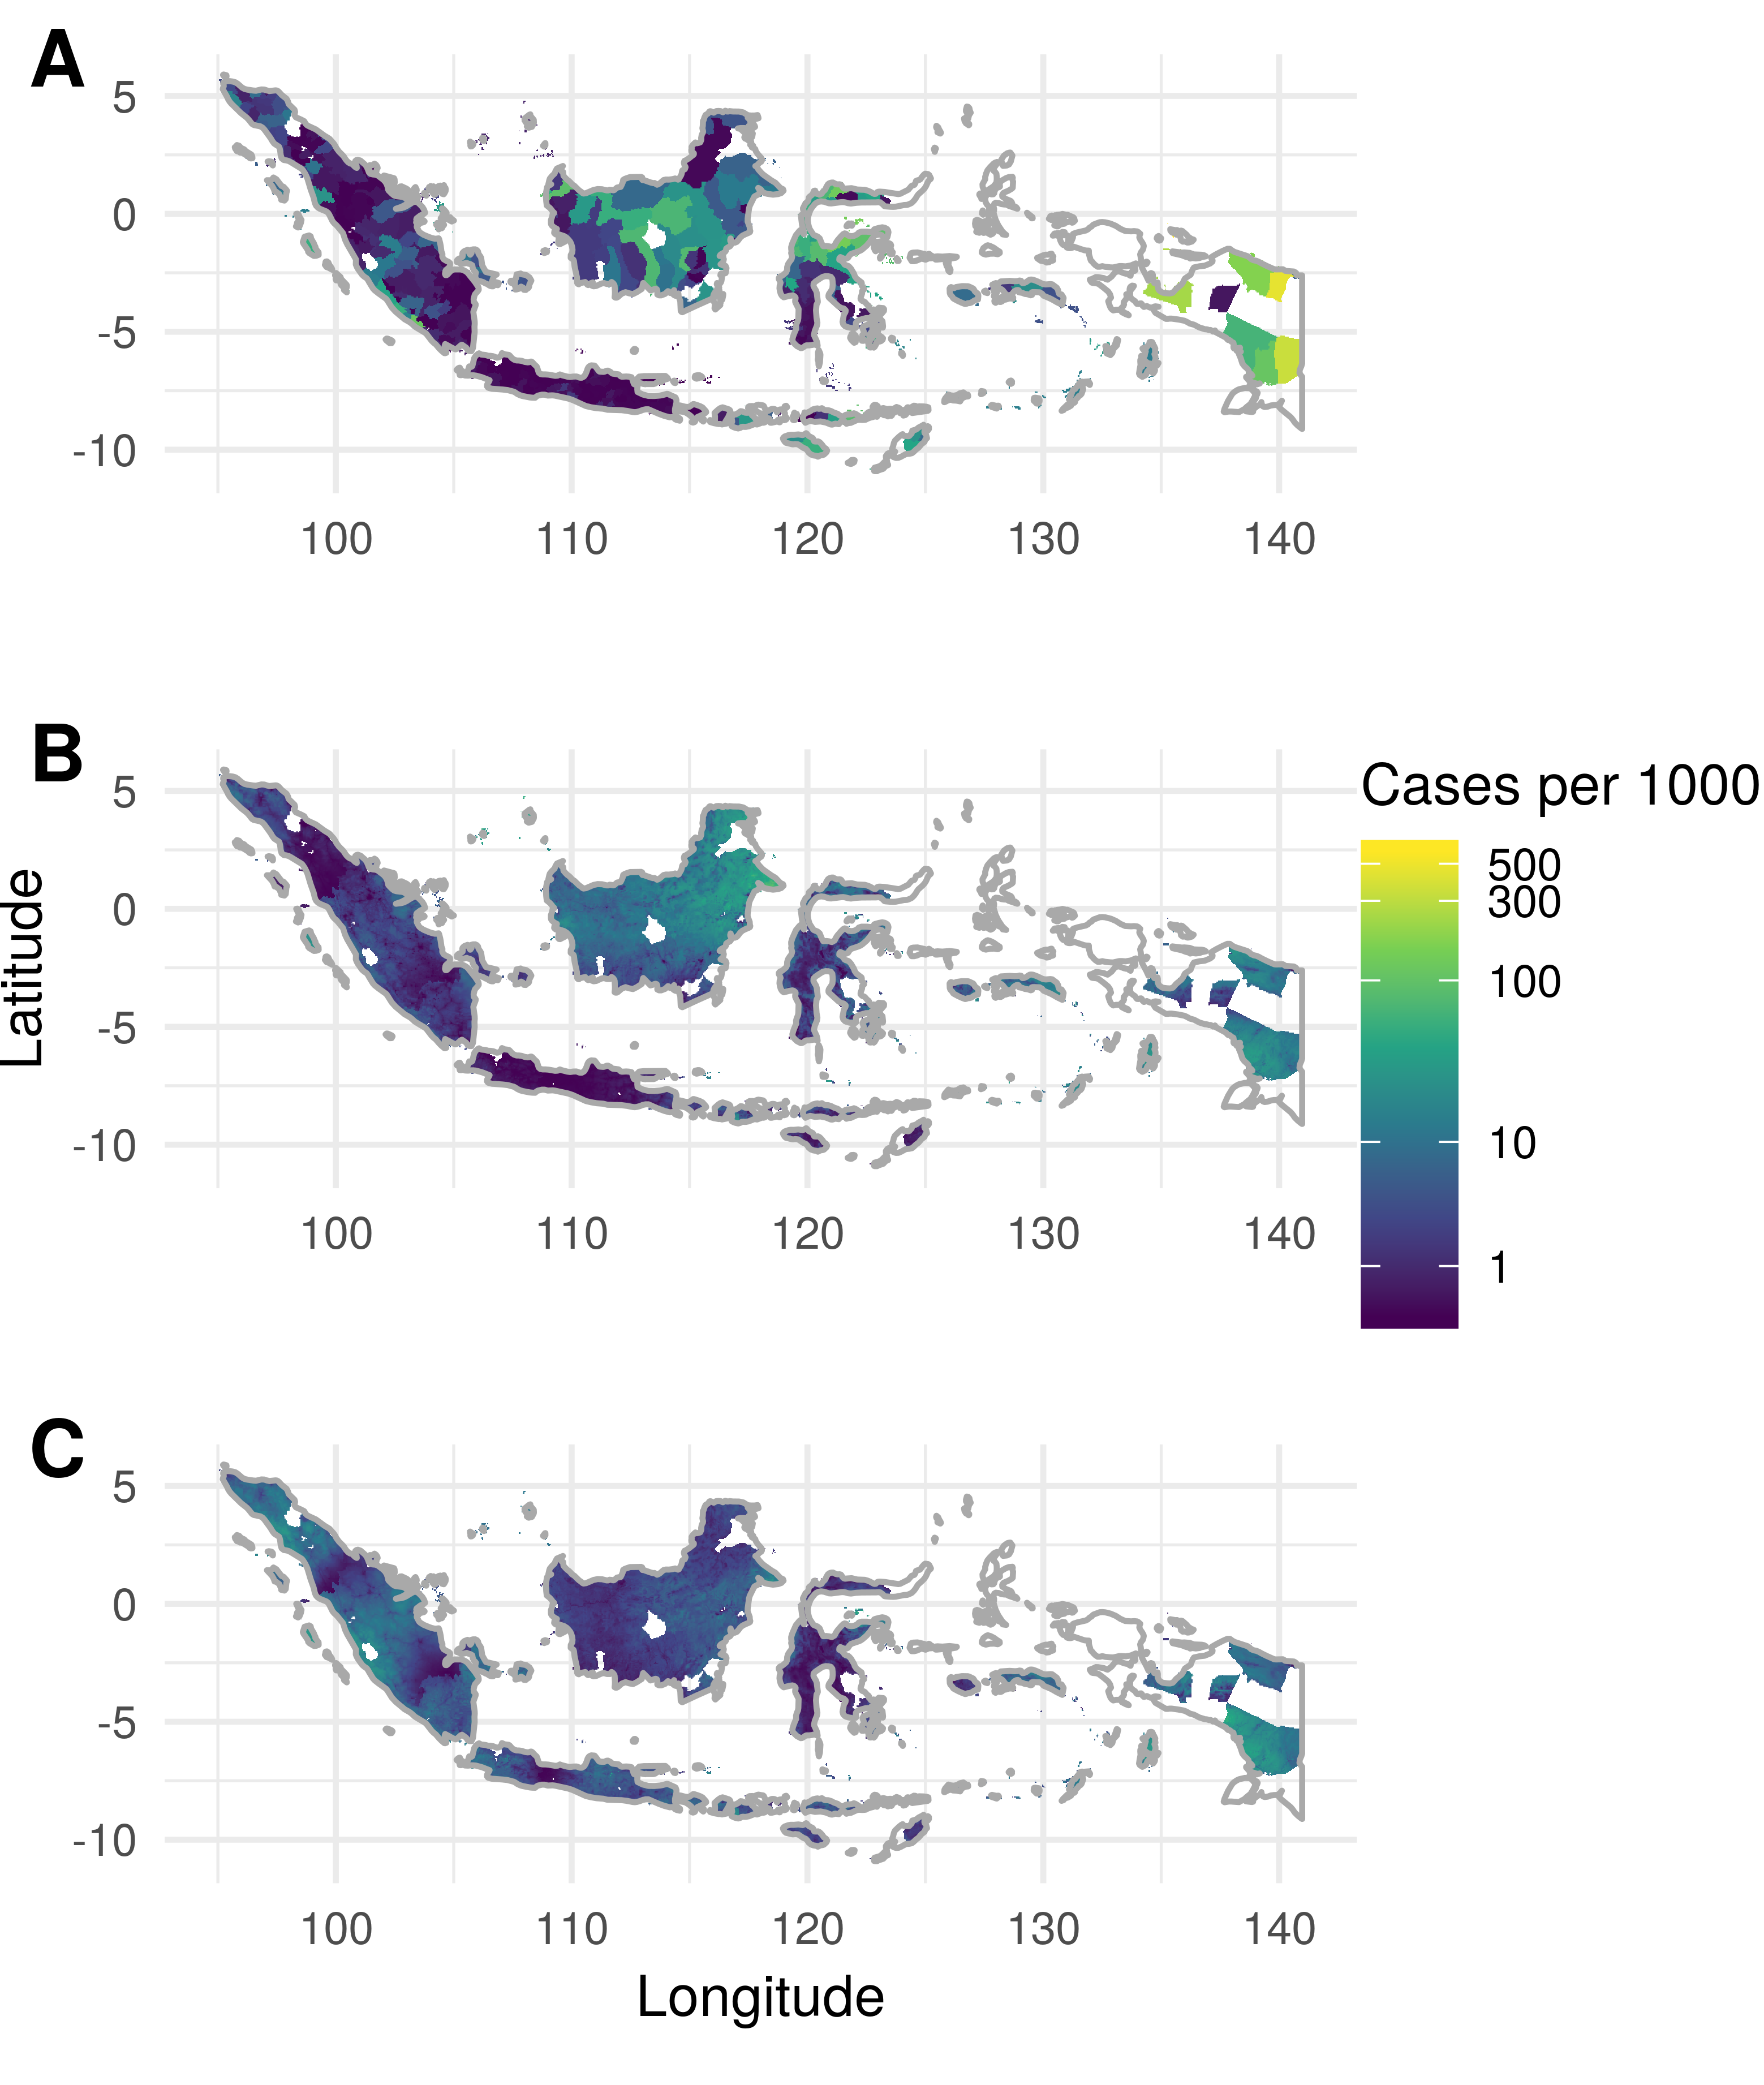
\includegraphics[width = 0.7\textwidth]{figures/idn_both_cv12_preds.png}
\caption{{\bf Input incidence data and predicted incidence maps. } 
The incidence (log10) data (top), predicted log10 incidence from the joint model for randomly sampled out-of-sample polygons (middle) and predicted log10 incidence from the joint model for spatially sampled out-of-sample polygons (bottom) for Indonesia. The values plotted for areas with no polygon data are the means across all cross-validation folds.
}
\label{predobsmapidn}
\end{figure}




\begin{figure}
% to be removed before submission
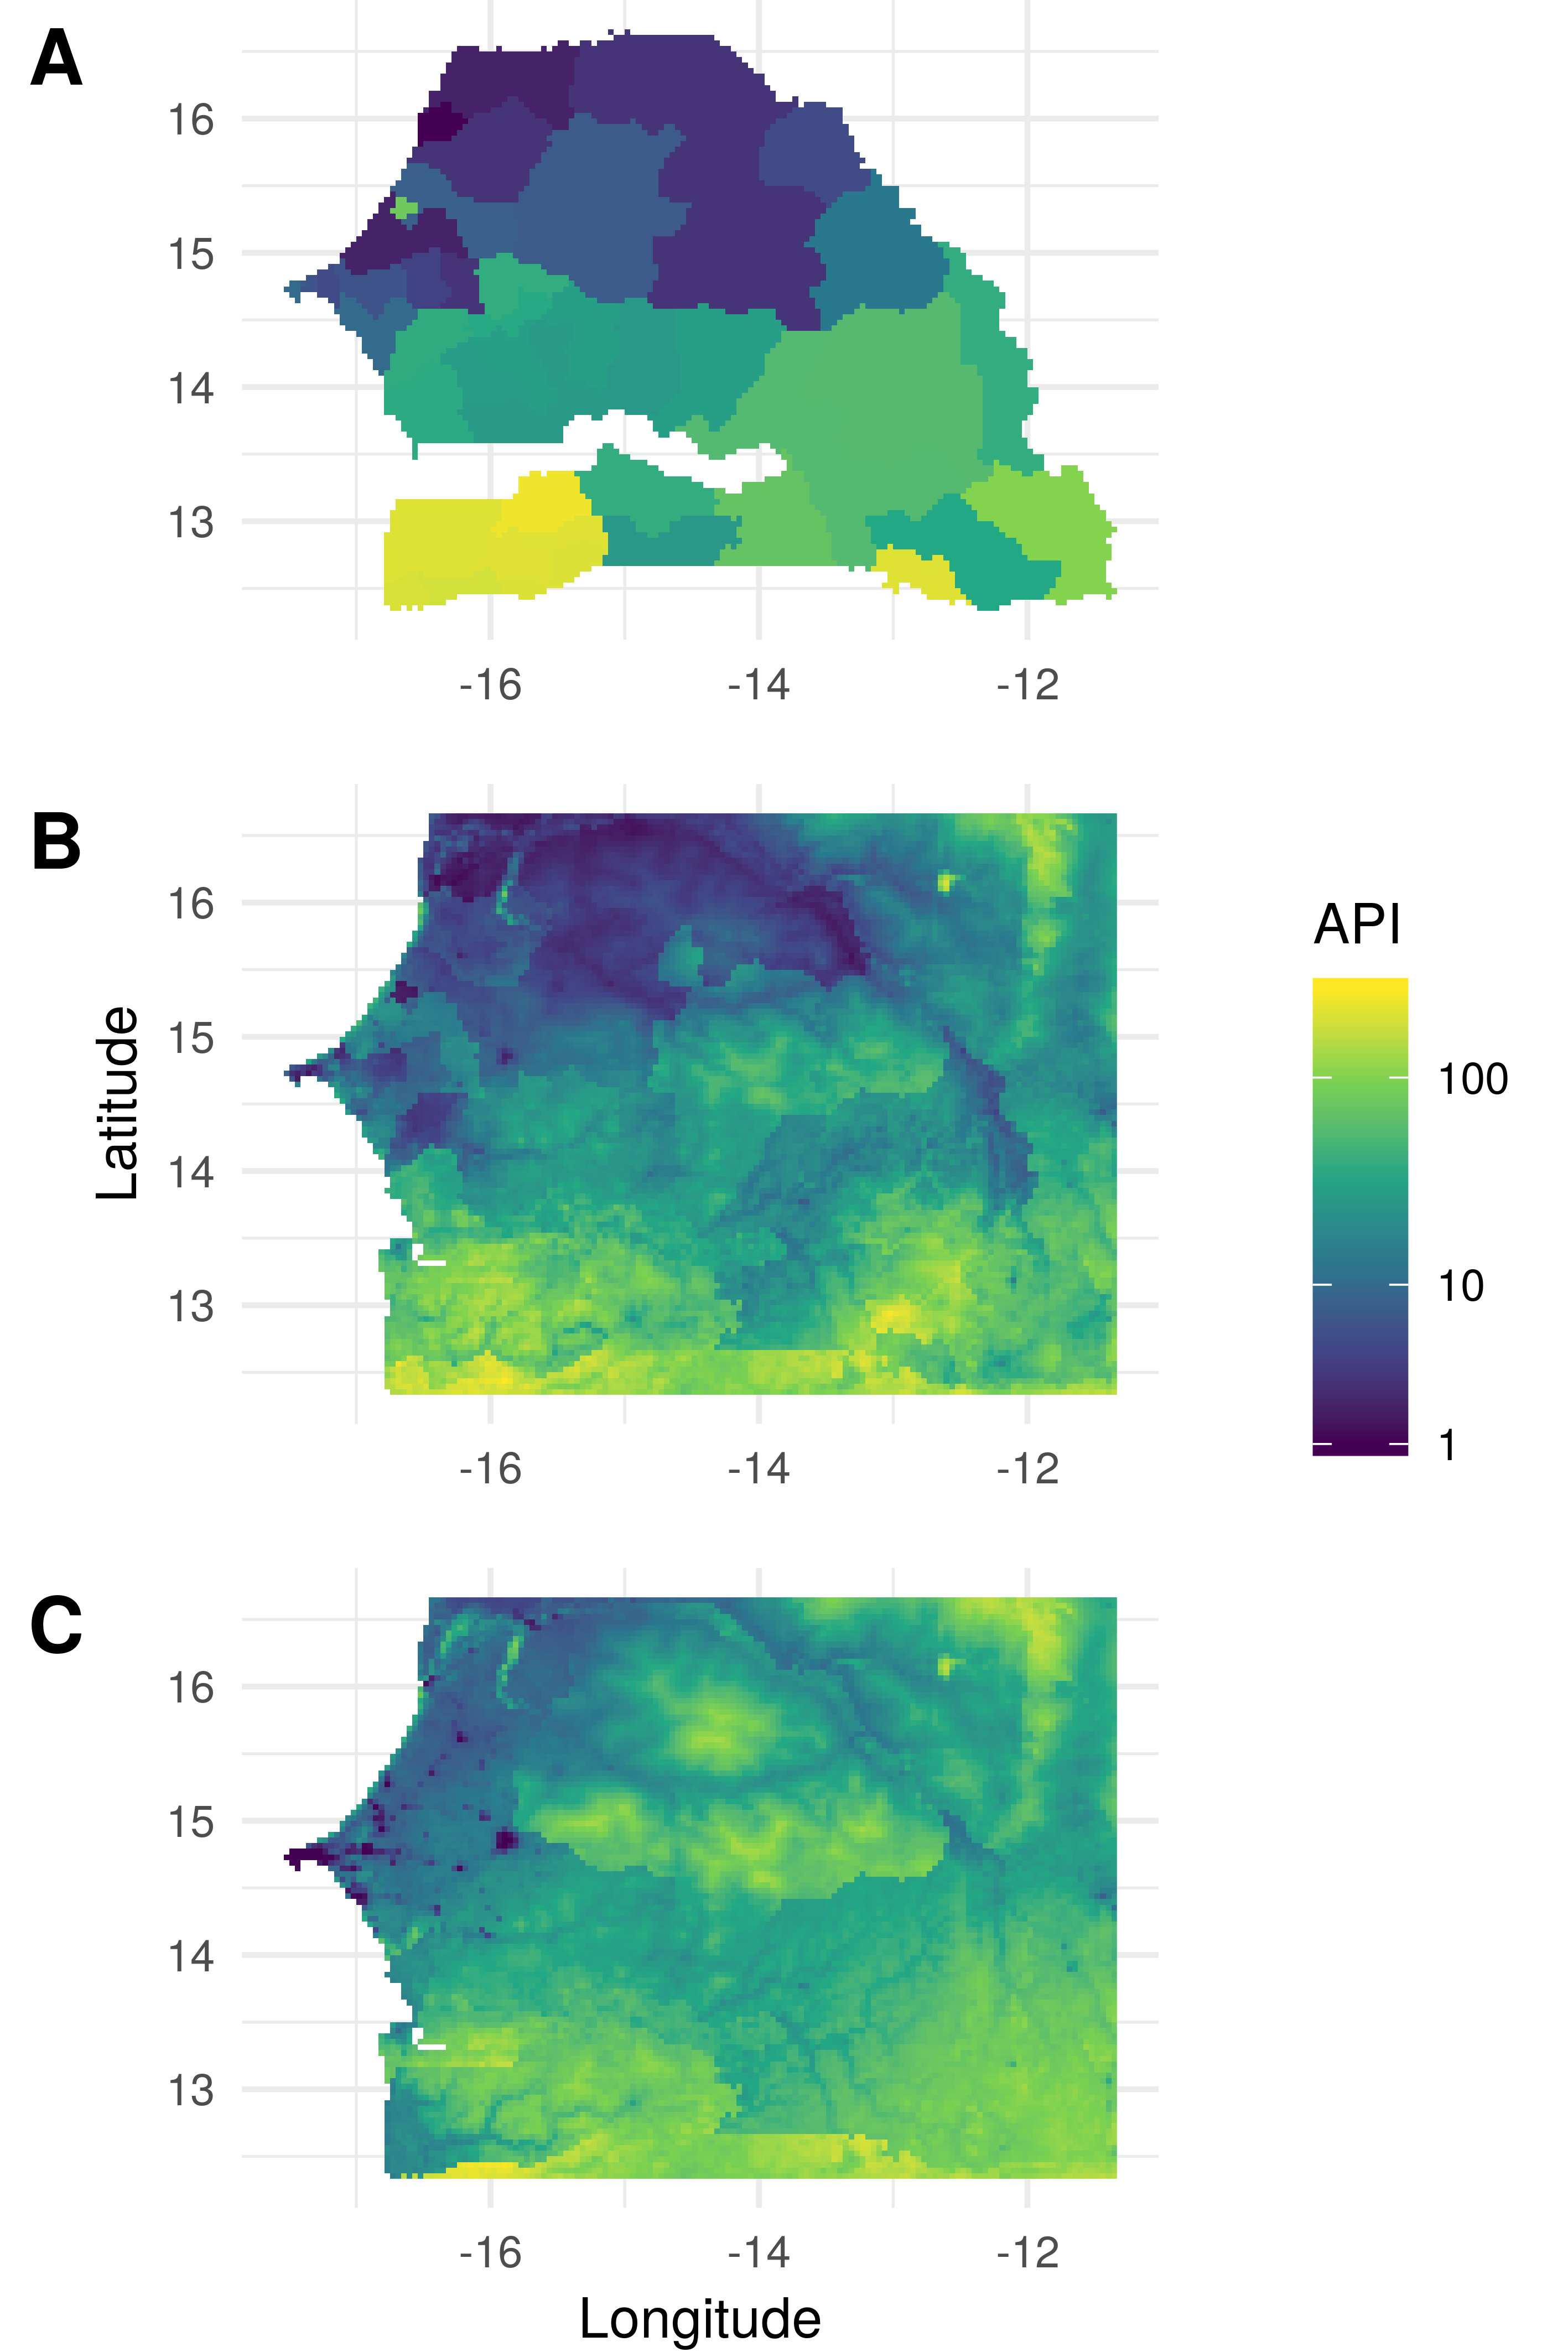
\includegraphics[width = 0.7\textwidth]{figures/sen_both_cv12_preds.png}
\caption{{\bf Input incidence data and predicted incidence maps. } 
The incidence (log10) data, predicted log10 incidence from the joint model for randomly sampled out-of-sample polygons (middle) and predicted log10 incidence from the joint model for spatially sampled out-of-sample polygons (bottom) for Senegal.
}
\label{predobsmapsen}
\end{figure}


% Results and Discussion can be combined.
%%%%%%%%%%%%%%%%%%%%%%%%%%%%%%%%%%%%%%%%%%%%%%%%%%%%%%%%%%%%%%%%%%%%%%%%%%%%%%%%%%%%%%%%%%%%%%%%%%%%%
\section*{Discussion}
%%%%%%%%%%%%%%%%%%%%%%%%%%%%%%%%%%%%%%%%%%%%%%%%%%%%%%%%%%%%%%%%%%%%%%%%%%%%%%%%%%%%%%%%%%%%%%%%%%%%%


%Summarise results

We have compared the predictive performance of a polygon-only model and a model that jointly learns from polygon incidence data and prevalence point-surveys.



%%%%%%%%%%%%%%%%%%%%%%%%%%%%%%%%%%%%%%%%%%%%%%%%%%%%%%%%%%%%%%%%%%%%%%%%%%%%%%%%%%%%%%%%%%%%%%%%%%%%%
\section*{Conclusion}
%%%%%%%%%%%%%%%%%%%%%%%%%%%%%%%%%%%%%%%%%%%%%%%%%%%%%%%%%%%%%%%%%%%%%%%%%%%%%%%%%%%%%%%%%%%%%%%%%%%%%





\section*{Supporting information}

% Include only the SI item label in the paragraph heading. Use the \nameref{label} command to cite SI items in the text.
%\paragraph*{S1 Fig.}
%\label{S1_Fig}
%{\bf Bold the title sentence.} Add descriptive text after the title of the item (optional).


\section*{Acknowledgments}
Thanks everyone.


\nolinenumbers

% Either type in your references using
% \begin{thebibliography}{}
% \bibitem{}
% Text
% \end{thebibliography}
%
% or
%
% Compile your BiBTeX database using our plos2015.bst
% style file and paste the contents of your .bbl file
% here. See http://journals.plos.org/plosone/s/latex for 
% step-by-step instructions.
% 
\bibliography{Malaria} 

%\begin{thebibliography}{10}


%\end{thebibliography}



\end{document}

